%\chapter{\Objectivetwoname}
\chapter{Experimental Setup and Results}\label{ch:chapter_3}

\section{Experimental Setup and Results}

To demonstrate that the hybrid model proposed as a result of this research enhances the performance of an already existing interpretability technique in the state of the art, firstly, we proceed to assess the performance of the interpretability techniques RawAtt, Rollout, and AttCat on the BERT, Roberta, and Distilbert models using the VisualMRC database. 

For this purpose, precision@k is calculated by varying k from 4 to 380. This range is chosen based on an exploratory analysis of the data, revealing that the contexts of samples in the VisualMRC database have a variable number of tokens ranging from 4 to 380 tokens. 

This is done with the objective of plotting precision@k curves versus k, aiming to identify the elbow point for each case. The elbow point represents the smallest k that yields the highest possible precision@k. It is important to note that a lower elbow point indicates better performance for the interpretability technique. The results of this experiment are presented in figures \ref{fig:PKbert}, \ref{fig:PKdistilbert} and \ref{fig:PKroberta}. 

\newpage

\begin{figure}[H]
    \centering%width=0.5\linewidth
    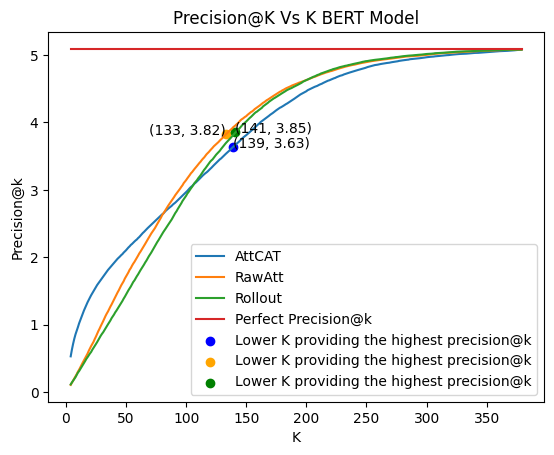
\includegraphics[width=0.75\linewidth]{Figures/Experimental Setup/Codo_BERT_VMRC.png}
    \caption{Precision@k Vs K in BERT Model}
    \label{fig:PKbert}
\end{figure}

%\newpage

\begin{figure}[H]
    \centering%width=0.5\linewidth
    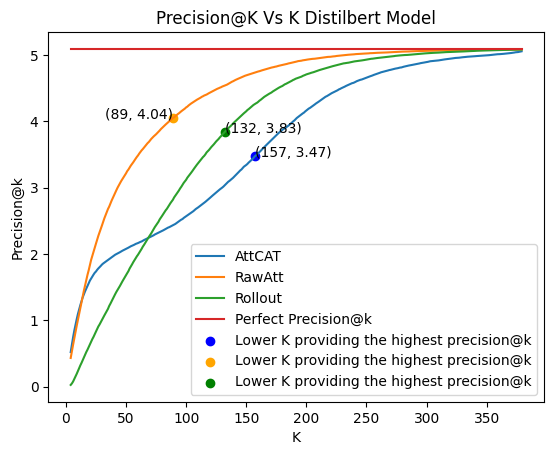
\includegraphics[width=0.75\linewidth]{Figures/Experimental Setup/Codo_Distilbert_VMRC.png}
    \caption{Precision@k Vs K in Distilbert Model}
    \label{fig:PKdistilbert}
\end{figure}

%\newpage


\begin{figure}[H]
    \centering%width=0.5\linewidth
    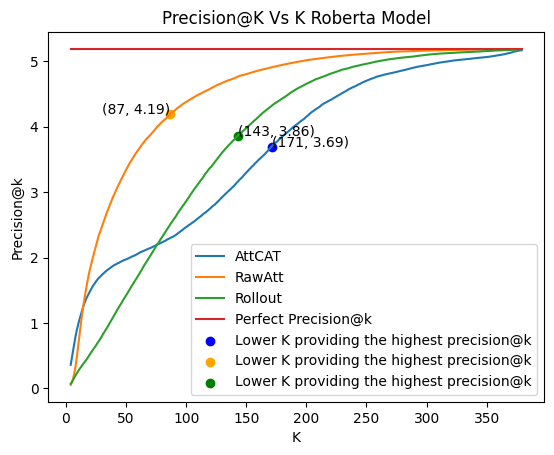
\includegraphics[width=0.75\linewidth]{Figures/Experimental Setup/Codo_Roberta_VMRC.png}
    \caption{Precision@k Vs K in Roberta Model}
    \label{fig:PKroberta}
\end{figure}

%\newpage

Furthermore, by normalizing the curves presented earlier, we calculate the area under the curve. It's important to note that an area under the curve closer to 1 indicates better performance for the interpretability technique, while an area closer to zero suggests poorer performance. The results of this experiment are depicted in figures \ref{fig:aucbert}, \ref{fig:aucdistilbert} and \ref{fig:aucroberta}.

\newpage

\begin{figure}[H]
    \centering%width=0.7\linewidth
    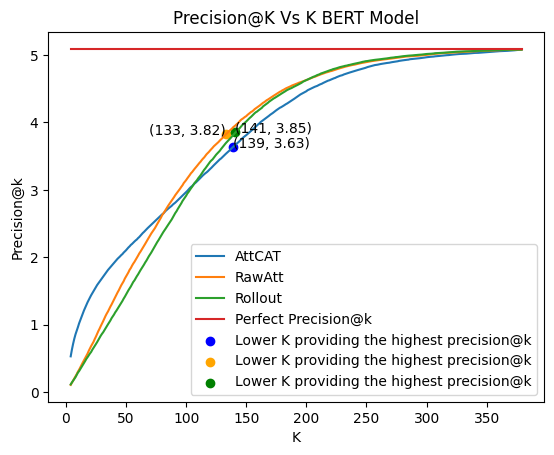
\includegraphics[width=0.75\linewidth]{Figures/Experimental Setup/Codo_BERT_VMRC.png}
    \caption{Area Under Curve in BERT Model}
    \label{fig:aucbert}
\end{figure}

\begin{figure}[H]
    \centering%width=0.7\linewidth
    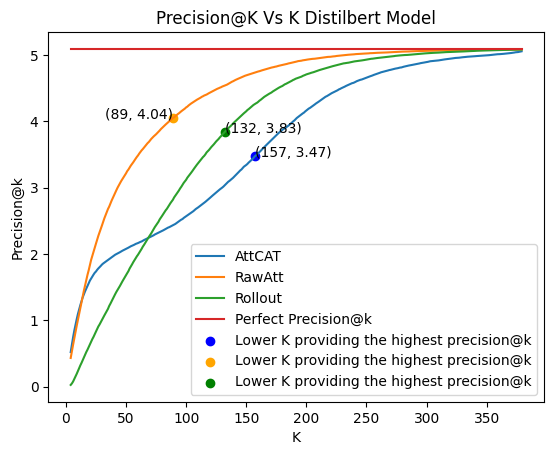
\includegraphics[width=0.75\linewidth]{Figures/Experimental Setup/Codo_Distilbert_VMRC.png}
    \caption{Area Under Curve in Distilbert Model}
    \label{fig:aucdistilbert}
\end{figure}

\begin{figure}[h!]
    \centering%width=0.7\linewidth
    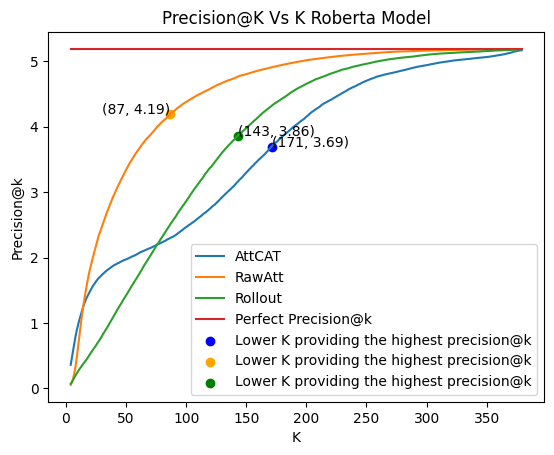
\includegraphics[width=0.75\linewidth]{Figures/Experimental Setup/Codo_Roberta_VMRC.png}
    \caption{Area Under Curve in Roberta Model}
    \label{fig:aucroberta}
\end{figure}


The previous results demonstrate that RawAtt is the interpretability technique that performs best on the VisualMRC database for the BERT, Distilbert, and Roberta models. This is evidenced by providing the highest area under the curve for all three models and, additionally, the lowest elbow point k for each of them.
 \newpage


\subsection{Improving the performance of RawAtt}


Now, considering that the VisualMRC database provides information about the semantic class in which the answer is found in each sample, the same previous experiment is conducted, but stratifying by semantic class. The goal is to determine which model performs best in each semantic class for the RawAtt interpretability technique. This approach aims to propose a hybrid model that surpasses the performance of the RawAtt interpretability technique on the three models experimented with earlier. The results of this experiment are summarized in table \ref{tabla:bestmodel}.

\begin{table*}[ht]
    \centering
    \caption{Best Model in Every Semantic Class}
    \label{tabla:bestmodel}
    \begin{tabularx}{\textwidth}{|X|c|c|c|c|}
        \hline
        \textbf{Semantic Class} & \textbf{Best Model} & \textbf{AUC} & \textbf{K} & \textbf{Precision@K} \\
        \hline
        Caption & Roberta & 0.90 & 73 & 3.29 \\
        Data & Roberta & 0.69 & 133 & 2.19 \\
        Heading/Title & Roberta & 0.86 & 92 & 4.52 \\
        List & Distilbert & 0.96 & 33 & 3.08 \\
        Other & Roberta & 0.91 & 68 & 3.28 \\
        Paragraph/Body & Roberta & 0.87 & 87 & 4.28 \\
        Picture & Roberta & 0.84 & 89 & 3.45 \\
        SubData & Distilbert & 0.97 & 35 & 5 \\
        Subtitle/Byline & Roberta & 0.87 & 92 & 4.78 \\
        \hline
    \end{tabularx}
\end{table*}


As shown in table \ref{tabla:bestmodel}, Distilbert is the model that performs best on the semantic classes List and SubData, while Roberta is the model that excels in the remaining semantic classes. Therefore, this information has been leveraged to propose a hybrid model that uses either Distilbert or Roberta based on the semantic class of the answer in the VisualMRC database. The aim is to enhance the performance of the RawAtt interpretability technique on the VisualMRC database.
\\\\
To demonstrate that indeed the proposed hybrid model improves the performance of the RawAtt interpretability technique on the VisualMRC database compared to the three models BERT, Distilbert, and Roberta, the same experiment proposed at the beginning of this section is conducted, but using the hybrid model. The results of this experiment are depicted in Figures \ref{fig:pkhybrid} and \ref{fig:auchybrid}. \newpage


\begin{figure}[H]
    \centering%width=0.7\linewidth
    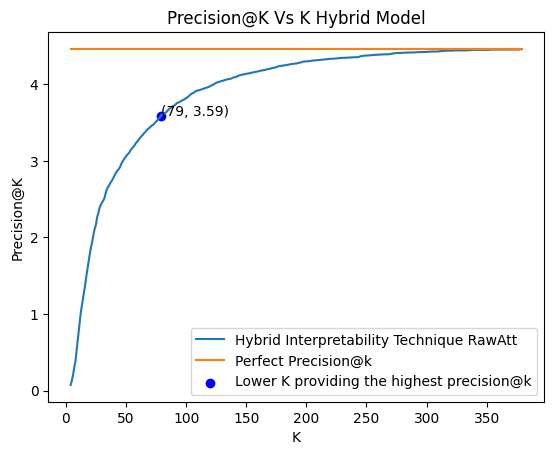
\includegraphics[width=0.75\linewidth]{Figures/Experimental Setup/RawAtt_Hybrid_Model_Codo.png}
    \caption{Precision@k Vs K in Hybrid Model}
    \label{fig:pkhybrid}
\end{figure}

\begin{figure}[H]
    \centering%width=0.7\linewidth
    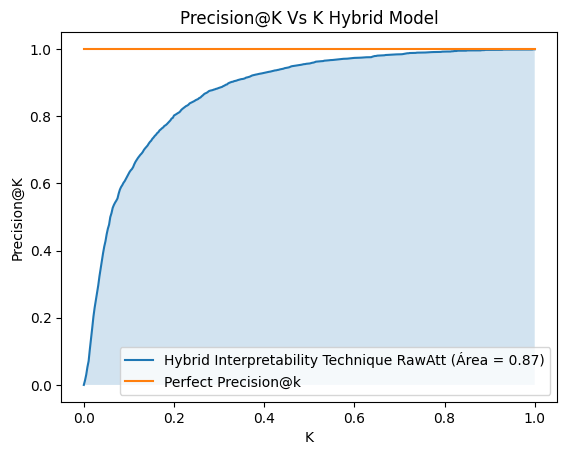
\includegraphics[width=0.75\linewidth]{Figures/Experimental Setup/RawAtt_Hybrid_Model_AUC.png}
    \caption{Area Under Curve in Hybrid Model}
    \label{fig:auchybrid}
\end{figure}

\newpage

As evident from Figures \ref{fig:pkhybrid} and \ref{fig:auchybrid}, while the hybrid model may not surpass the area under the curve of the precision@k vs k curve for the three models BERT, Roberta, and Distilbert, it does outperform these models in terms of performance. This is indicated by providing a lower elbow point k than the three aforementioned models, meaning it achieves a smaller k at the elbow point that yields the highest precision@k.

\subsection{Strengthening RawAtt}

On the other hand, through Monte Carlo simulations, wherein the experiment is repeated 10 times using different samples for both the three initial models and the hybrid model, it has been shown that the RawAtt interpretability technique using the hybrid model is more robust than using the other three models when faced with changes in the type of text in the sample. This is evident from Figures \ref{msbert}, \ref{msroberta}, \ref{msdistilbert}and \ref{mshybrid}, where the standard deviation of precision@k is much lower for the hybrid model than for the other three models. 

\begin{figure}[H]
    \centering%width=0.7\linewidth
    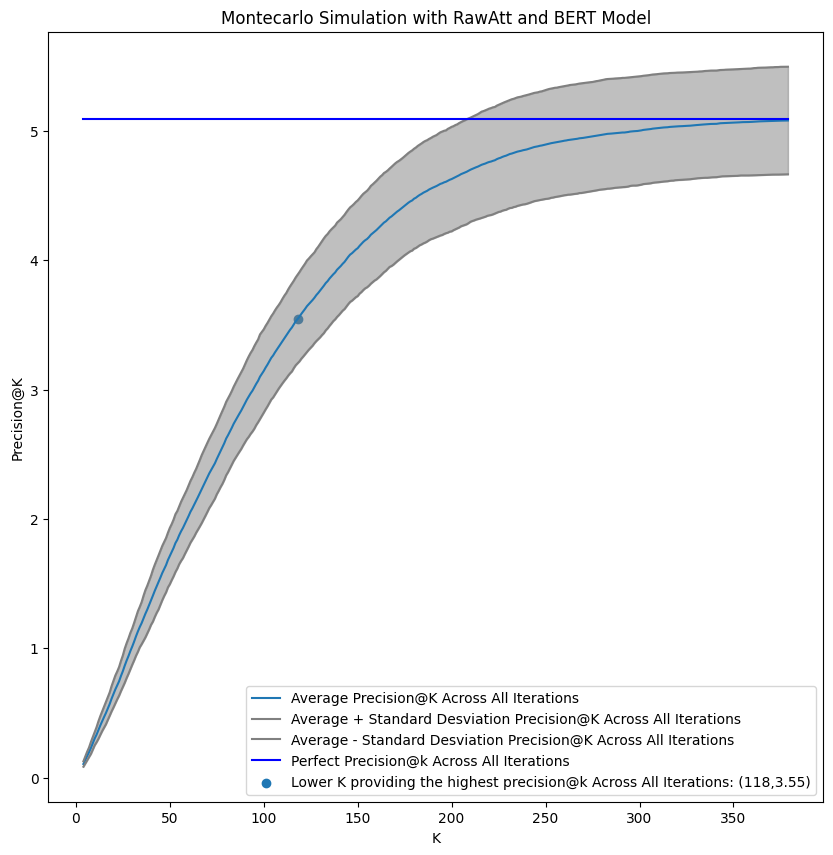
\includegraphics[width=0.75\linewidth]{Figures/Experimental Setup/Fill_Between_BERT_RawAtt.png}
    \caption{Standard Desviation of the precision@k of the RawAtt Interpretability Technique with BERT Model in a Montecarlo Simulation}
    \label{msbert}
\end{figure}


\begin{figure}[H]
    \centering%width=0.7\linewidth
    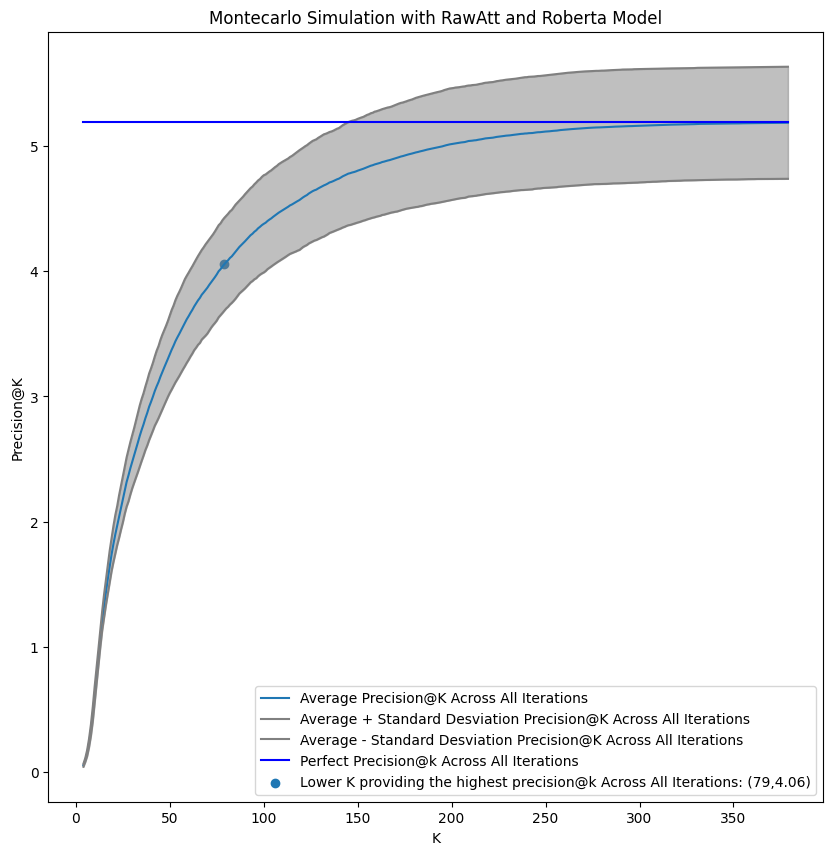
\includegraphics[width=0.75\linewidth]{Figures/Experimental Setup/Fill_Between_Roberta_RawAtt.png}
    \caption{Standard Desviation of the precision@k of the RawAtt Interpretability Technique with Roberta Model in a Montecarlo Simulation}
    \label{msroberta}
\end{figure}

\begin{figure}[H]
    \centering%width=0.7\linewidth
    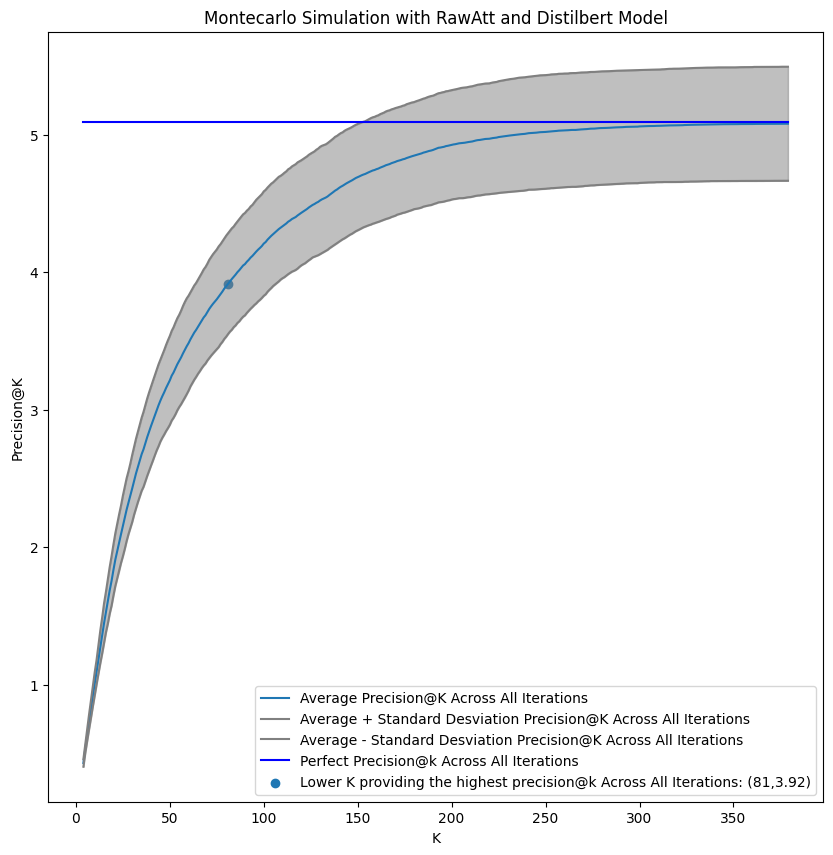
\includegraphics[width=0.75\linewidth]{Figures/Experimental Setup/Fill_Between_Distilbert_RawAtt.png}
    \caption{Standard Desviation of the precision@k of the RawAtt Interpretability Technique with Distilbert Model in a Montecarlo Simulation}
    \label{msdistilbert}
\end{figure}

\begin{figure}[H]
    \centering%width=0.7\linewidth
    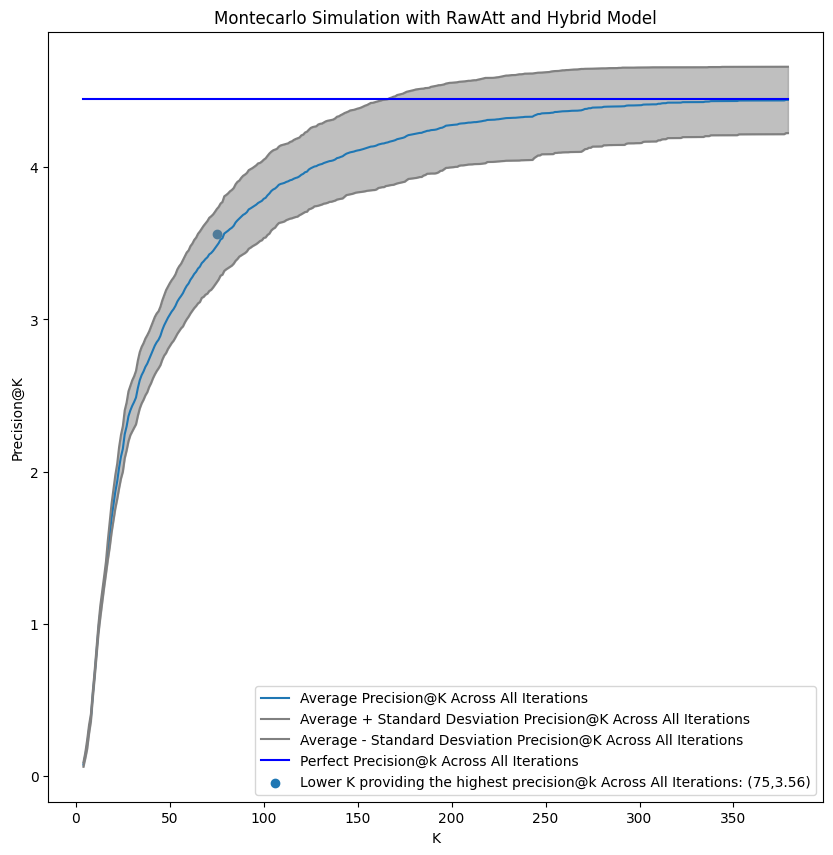
\includegraphics[width=0.75\linewidth]{Figures/Experimental Setup/Fill_Between_Hybrid_Model_RawAtt.png}
    \caption{Standard Desviation of the precision@k of the RawAtt Interpretability Technique with Hybrid Model in a Montecarlo Simulation}
    \label{mshybrid}
\end{figure}

Furthermore, the standard deviation of the elbow point k, i.e., the smallest k at which the highest precision@k is achieved, is much lower in the hybrid model than in the other three models. This is illustrated in Figure \ref{sdk}.

\newpage

\begin{figure}[h!]
    \centering%width=0.7\linewidth
    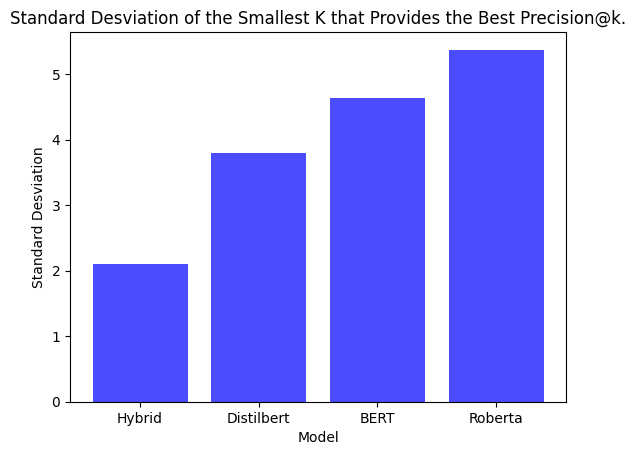
\includegraphics[width=\linewidth]{Figures/Experimental Setup/sd_k.png}
    \caption{Standard Desviation of the Smallest K that Provides the Best Precision@k}
    \label{sdk}
\end{figure}


\subsection{Database - Visual Machine Reading Comprehension}
\label{Database}


Introducded by \cite{visualmrc}, VisualMRC comprises over 30,000 question-answer pairs, providing abstractive answers for more than 10,000 document images sourced from diverse web page domains. This dataset is distinct from conventional visual question answering (VQA) datasets by placing a heightened emphasis on the development of natural language understanding and generation capabilities. Figure \ref{fig:visualmrc} shows an instance example of VisualMRC.

\newpage


\begin{figure}[h!]
    \centering%width=0.7\linewidth
    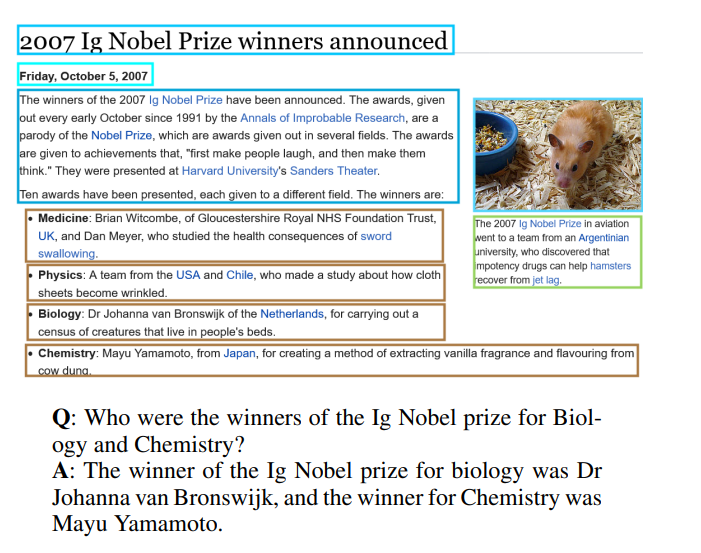
\includegraphics[width=\linewidth]{Figures/Preliminares/visualmrc_example.png}
    \caption{Example of the VisualMRC dataset \cite{visualmrc}}
    \label{fig:visualmrc}
\end{figure}


It is important to note that, for our experiments, we have only used those VisualMRC instances that are adapted to the  extractive question answering  task, that is, those instances in which the answer to the question is extractive from a context and not generative.

\newpage

\subsection{RawAtt Interpretability Technique and Hybrid Model Over VisualMRC Database}

As shown in Figure \ref{fig:sota}, multiple authors have demonstrated that the interpretability techniques based in attention weights alone are not reliable when assigning a relevance score to a token; however, we have performed an experiment to demonstrate that the RawAtt interpretability technique works well with our proposed hybrid model in the VisualMRC database. For this we have carried out the average drop experiment, which consists of finding the performance of the model as the most relevant tokens are removed according to the interpretability technique, in order to be able to observe whether the most relevant tokens for the model are actually yields the interpretability technique actually are. This is ilustrated in Figure \ref{fig:averagedrop}:

\begin{figure}[H]
    \centering%width=0.7\linewidth
    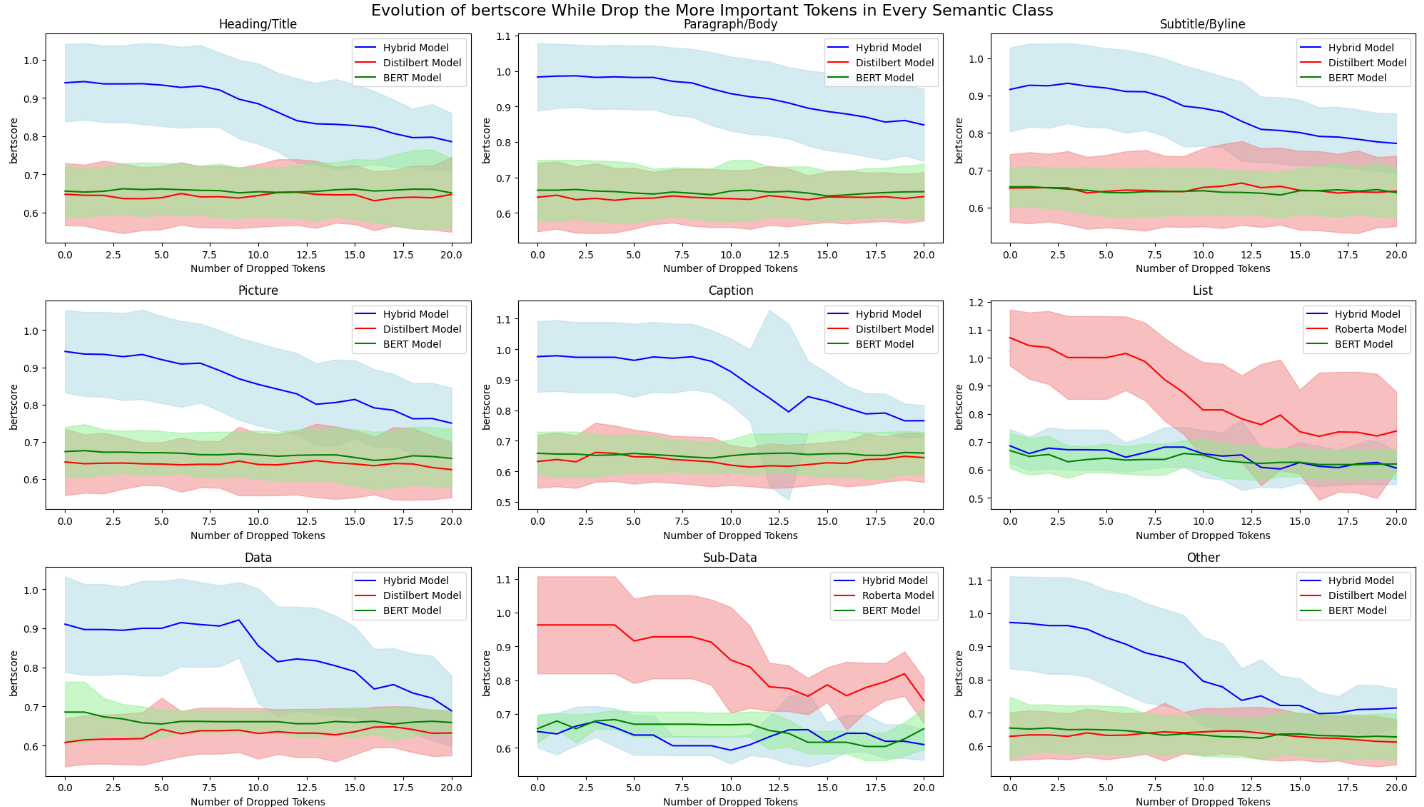
\includegraphics[width=\linewidth]{Figures/Experimental Setup/average_drop.png}
    \caption{Evolution of BertScore While Drop the More Important Tokens in Every Semantic Class}
    \label{fig:averagedrop}
\end{figure}

As is evident in Figure \ref{fig:averagedrop}, in almost all semantic classes, our hybrid model works best with the RawAtt interpretability technique; Since as you can see, as the most relevant tokens for the model are removed, its performance decreases. This excepts the List and Sub-Data semantic classes; but this is because the VisualMRC database does not have a significant number of instances adaptable to the task of extractive question answering in these two semantic classes: Sub-Data (6) and List(13).

\newpage

Figure \ref{fig:bert_precision} shows that with our hybrid model, we outperformance in BERT score average drop to the other models in almost all semantic classes (less in Sub-Data and List semantic classes), but in this two classes (so as in all the semantic classes), with our hybrid model we outperformance to the other models in precision@k.


\begin{figure}[H]
    \centering%width=0.7\linewidth
    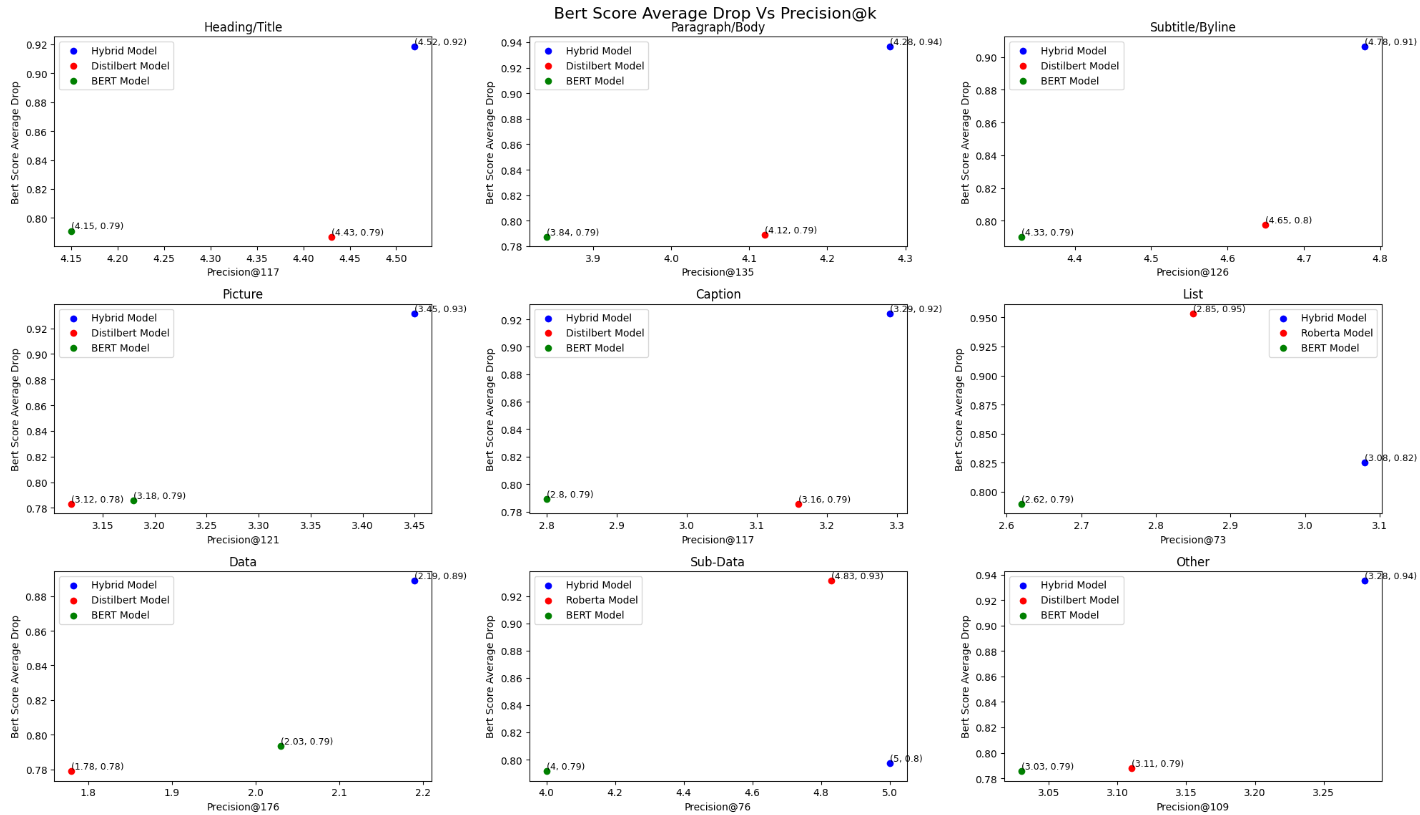
\includegraphics[width=\linewidth]{Figures/Experimental Setup/bert_precision.png}
    \caption{BERT Score Average Drop Vs Precision@k}
    \label{fig:bert_precision}
\end{figure}


As can be seen in figure \ref{fig:important_words},  in almost all the semantic classes (less List and Sub-Data semantic classes), for the model is very important the special tokens, to identify where a sequence begins ( <S> ) and where a sequence finishes ( </S> ). Also, for the model is very important the interrogative words and the interrogative sign, to identify what the user is asking. 


\begin{figure}[H]
    \centering%width=0.7\linewidth
    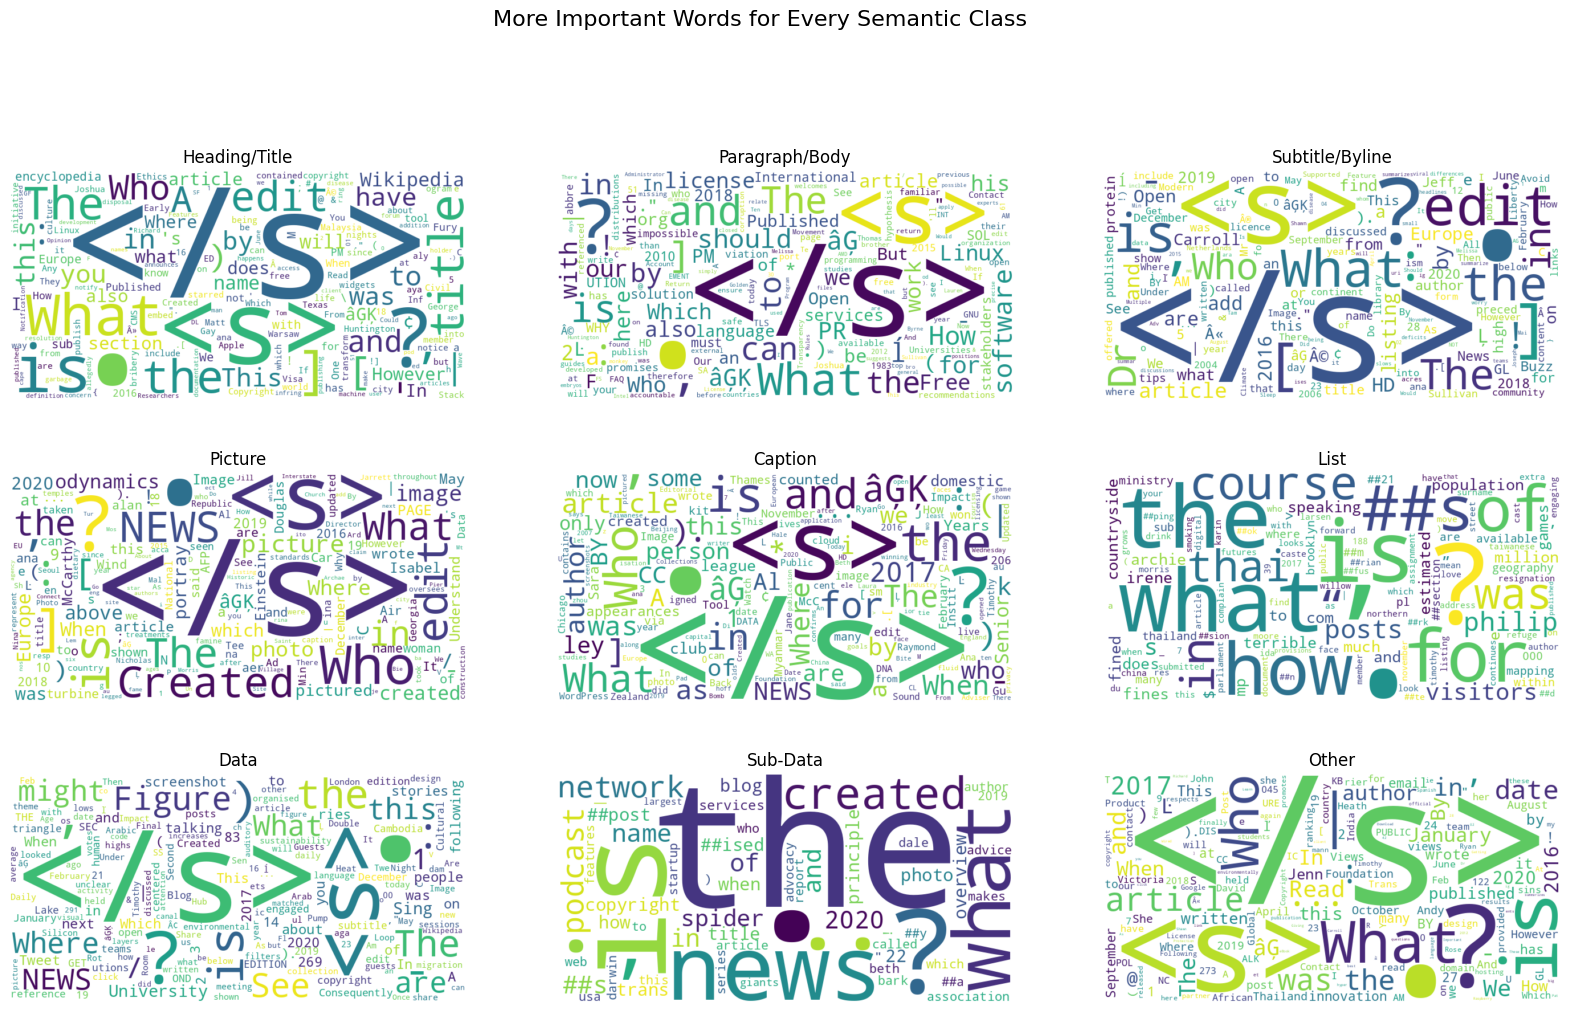
\includegraphics[width=\linewidth]{Figures/Experimental Setup/relevance_words.png}
    \caption{More Important Words for Every Semantic Class Agree to RawAtt}
    \label{fig:important_words}
\end{figure}

